\section{Basics of graph theory}

ในส่วนนี้ จะกล่าวถึงนิยามต่างๆ ที่เป็นพื้นฐานของทฤษฎีกราฟ

\begin{definition}
    \emph{กราฟ} (graph) คือคู่อันดับ $G=(V,E)$ โดยที่ $V$ เป็นเซตของ\emph{จุดยอด} (vertices\footnote{หากเป็นเอกพจน์ จะเขียนว่า vertex}) และ $E$ เป็นเซตของ\emph{เส้นเชื่อม} (edges) โดยแต่ละเส้นนั้นเป็น subset ของ $V$ ที่มีสมาชิก 2 ตัว
\end{definition}
ทั้งนี้ อาจจะเรียก vertices ว่า nodes ก็ได้

\begin{example}
กราฟในรูป~\ref{fig:map-graph} ประกอบไปด้วย vertices และ edges ดังนี้
\begin{align*}
    V &= \set{1,2,3,4} \\
    E &= \set{\set{1,2}, \set{1,4}, \set{2,3}, \set{2,4}, \set{3,4}}
\end{align*}
\end{example}
%
สังเกตว่า เส้นในกราฟนั้นสามารถเขียนได้เป็น subsets ของ $V$ ซึ่งแต่ละ subset นั้นมีสมาชิก 2 ตัว เช่น เส้นที่เชื่อมจุด 1 และ 2 จะเป็น subset $\set{1,2}\subseteq V$ \enskip เหตุผลที่เราเขียนแต่ละเส้นเป็นเซตนั้น เนื่องจากลำดับของจุดไม่สำคัญ กล่าวคือ หากจะเขียนแทนเส้นด้วยเซต $\set{2,1}$ ก็ยังคงหมายถึงเส้นที่เชื่อมจุด 1 และ 2 เช่นเดิม

\begin{definition}
ให้ $u,v\in V$ \enskip เรียก $u$ ว่า\emph{ประชิด} (adjacent) กับ $v$ [denoted $u\sim v$] หาก $\set{u,v}\in E$
\end{definition}
%
\begin{example}
จากกราฟในรูปที่~\ref{fig:map-graph} จะได้ว่า $4\sim 2$ เนื่องจาก $\set{4,2}\in E$ แต่ $1\not\sim 3$
\end{example}

\begin{definition}
ให้ $e=\set{u,v}$ เป็น edge ในกราฟ \enskip เรียก $e$ ว่า \emph{incident with} $u$ (และ $v$)
\end{definition}
นั่นคือ แต่ละเส้นในกราฟจะ incident with จุดปลายแต่ละข้างของเส้นนั้นๆ

\begin{example}
จากกราฟในรูปที่~\ref{fig:map-graph} จะได้ว่าเส้น $\set{1,4}$ is incident with vertex 1.
\end{example}

\begin{definition}
ให้ $v\in V$ \enskip \emph{ดีกรี} (degree) ของ $v$ [denoted $\deg(v)$] คือจำนวนเส้นที่ incident with $v$
\end{definition}
นั่นคือ degree ของแต่ละจุด คือจำนวน edges ที่ต่ออยู่กับจุดนั้นๆ

\begin{example}
จากกราฟในรูปที่~\ref{fig:map-graph} จะได้ว่า $\deg(1)=2$ และ $\deg(2)=3$
\end{example}

จากนิยามต่างๆ ที่กล่าวมาข้างต้น เราสามารถพิสูจน์คุณสมบัติแรกของกราฟได้ดังนี้
\begin{lemma}
ให้ $G=(V,E)$ \enskip $\sum_{v\in V}{\deg(v)}=2|E|$
\begin{pf}
ในที่นี้ จะใช้ combinatorial proof โดยกำหนด $S\triangleq\set{(u,e)\mid\text{$e$ is incident with $u$}}$ เป็นเซตที่เราจะนับจำนวนสมาชิก \enskip เซตนี้เป็นเซตของคู่อันดับ ที่ตัวหน้าของคู่อันดับเป็น vertex ในกราฟ และตัวหลังของคู่อันดับเป็นเส้นที่ต่ออยู่กับ vertex นั้นๆ

ถัดไป จะทำการคำนวณ $|S|$ โดยสองวิธี
\begin{enumerate}
\item จะเห็นว่า แต่ละจุด $v$ ในกราฟ จะก่อให้เกิดคู่อันดับใน $S$ ทั้งสิ้น $\deg(v)$ คู่อันดับ โดยแต่ละคู่อันดับจะเป็นแต่ละเส้นที่ incident with $v$ \enskip กล่าวอีกนัยหนึ่ง $\deg(v)$ คือจำนวนสมาชิกของ $S$ โดยที่ตัวหน้าของคู่อันดับเป็น $v$ \enskip เมื่อรวม degrees ของทุกๆ จุดในกราฟ จะได้จำนวนสมาชิกทั้งหมดของ $S$ กล่าวคือ $|S|=\sum_{v\in V}{\deg(v)}$
\item จะเห็นว่า แต่ละเส้น $e=\set{u,v}$ ในกราฟ จะก่อให้เกิดคู่อันดับใน $S$ ทั้งสิ้น 2 คู่อันดับ ได้แก่ $(u,e)$ และ $(v,e)$ \enskip ดังนั้น จำนวนสมาชิกทั้งหมดของ $S$ ย่อมเป็นสองเท่าของจำนวนเส้นในกราฟ กล่าวคือ $|S|=2|E|$
\end{enumerate}
เนื่องจากเราสามารถนับจำนวนสมาชิกของ $S$ ได้สองวิธีที่แตกต่างกันข้างต้น จึงสรุปได้ว่า จำนวนสมาชิกที่นับได้ในแต่ละวิธีนั้นย่อมเท่ากัน นั่นคือ $\sum_{v\in V}{\deg(v)}=2|E|$
\end{pf}
\end{lemma}
%
\begin{example}
จากกราฟในรูปที่~\ref{fig:map-graph} จะได้ว่า เซต $S$ ใน lemma ข้างต้นเป็นเซต
\begin{align*}
\{
& (1,\set{1,2}),(2,\set{1,2}), (1,\set{1,4}),(4,\set{1,4}), \\
& (2,\set{2,3}),(3,\set{2,3}), (2,\set{2,4}),(4,\set{2,4}), \\
& (3,\set{3,4}),(4,\set{3,4})
\}
\end{align*}
\end{example}

\begin{definition}
ให้ $G=(V,E)$ \enskip \emph{แนวเดิน} (walk) คือลำดับของ vertices โดยที่แต่ละ vertex ในลำดับ ต้อง adjacent กับ vertex ตัวถัดไปในลำดับ \enskip ความยาวของ walk คือจำนวนครั้งที่มีการเปลี่ยนผ่านจุดในลำดับ ซึ่งจะน้อยกว่าความยาวของลำดับนั้นๆ อยู่ 1
\end{definition}
นั่นคือ walk เป็นการเดินไปมาในกราฟ โดยเริ่มจากจุดใดจุดหนึ่ง และเปลี่ยนจุดไปเรื่อยๆ โดยเดินตามเส้นที่ต่ออยู่กับจุดปัจจุบัน

\begin{example}
จากกราฟในรูปที่~\ref{fig:map-graph} ลำดับของ vertices ต่อไปนี้เป็น walks:
\begin{itemize}
\item $1,2,4,3$ เป็น walk ที่มีความยาว 3
\item $1,4,2,3,4$ เป็น walk ที่มีความยาว 4
\item $1,2,1,2,3,4,2,1,4$ เป็น walk ที่มีความยาว 8
\item $3$ เป็น walk ที่มีความยาว 0
\end{itemize}
\end{example}

\begin{definition}
\emph{วิถี} (path) คือ walk ที่ไม่มี vertex ซ้ำในลำดับ
\end{definition}
%
\begin{example}
จากกราฟในรูปที่~\ref{fig:map-graph} ลำดับของ vertices ต่อไปนี้เป็น paths:
\begin{itemize}
\item $1,2,4,3$ เป็น path ที่มีความยาว 3
\item $3$ เป็น path ที่มีความยาว 0
\end{itemize}
\end{example}

\begin{exercise}
กราฟในรูปที่~\ref{fig:map-graph} มี walks จากจุด 1 ไปยังจุด 3 ทั้งสิ้นเป็นจำนวนเท่าใด
\end{exercise}

\begin{exercise}
กราฟในรูปที่~\ref{fig:map-graph} มี paths จากจุด 1 ไปยังจุด 3 ทั้งสิ้นเป็นจำนวนเท่าใด
\end{exercise}

\begin{definition}
ให้ $u,v\in V$ \enskip เรียก $u$ ว่า\emph{เชื่อมโยงกับ} (connected to) $v$ หากมี path จาก $u$ ไป $v$
\end{definition}
%
\begin{example}
จากกราฟในรูปที่~\ref{fig:map-graph}, vertex 1 is connected to vertex 3, and vertex 4 is connected to itself.
\end{example}

\begin{definition}
เรียกกราฟว่า\emph{เชื่อมต่อ} (connected) หาก $\forall u,v\in V \exists\,\text{path จาก $u$ ไป $v$}$
\end{definition}
%
\begin{example}
กราฟในรูปที่~\ref{fig:map-graph} เป็น connected graph
\end{example}
%
\begin{example}
กราฟในรูปที่~\ref{fig:disconnected-graph} เป็น disconnected graph เนื่องจากไม่มี path จากจุด 2 ไปยังจุด 5
\begin{figure}
\centering
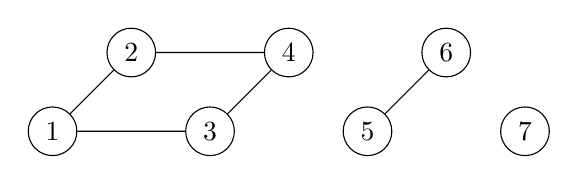
\begin{tikzpicture}
\node[circle,draw] (1) at (0,0) {1};
\node[circle,draw] (2) at (1,1) {2};
\node[circle,draw] (3) at (2,0) {3};
\node[circle,draw] (4) at (3,1) {4};
\node[circle,draw] (5) at (4,0) {5};
\node[circle,draw] (6) at (5,1) {6};
\node[circle,draw] (7) at (6,0) {7};
\draw (1) -- (2) -- (4) -- (3) -- (1);
\draw (5) -- (6);
\end{tikzpicture}
\caption{A disconnected graph}
\label{fig:disconnected-graph}
\end{figure}
\end{example}

\subsection{Common graphs}

กราฟที่พบเห็นบ่อย มีดังนี้

\begin{definition}
ให้ $n$ เป็นจำนวนเต็มบวก \enskip \emph{กราฟแบบบริบูรณ์} (complete graph) $K_n$ คือกราฟที่มี $n$ vertices และมี edge เชื่อมทุกคู่ของ vertices ที่เป็นไปได้
\end{definition}
%
\begin{example}
กราฟต่อไปนี้เป็น $K_5$ ซึ่งมีทั้งสิ้น 5 vertices และ 10 edges
\begin{center}
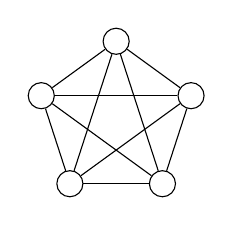
\begin{tikzpicture}
\foreach \i in {0,...,4} {
    \node[circle,draw] (\i) at (90-72*\i:1) {};
    \foreach \j in {0,...,\i} {
        \ifnum\i=\j\relax\else
        \draw (\i) -- (\j);
        \fi
    }
}
\end{tikzpicture}
\end{center}
\end{example}
เนื่องจาก $K_n$ มี $n$ vertices และมีเส้นเชื่อมทุกคู่จุดที่เป็นไปได้ จะได้ว่า จำนวน edges ใน $K_n$ มีค่าเป็น $\binom{n}{2}=\frac{n(n-1)}{2}$

\begin{definition}
\emph{กราฟว่าง} (empty graph) คือกราฟที่ไม่มี edge เลย
\end{definition}
%
\begin{example}
กราฟต่อไปนี้เป็น empty graph ที่มี 5 vertices
\begin{center}
\begin{tikzpicture}
\foreach \i in {0,...,4} {
    \node[circle,draw] (\i) at (90-72*\i:1) {};
}
\end{tikzpicture}
\end{center}
\end{example}

\begin{definition}
ให้ $n$ เป็นจำนวนเต็มบวก \enskip \emph{กราฟเส้น} (line graph) $L_n$ คือกราฟที่มี $n$ vertices และมี $n-1$ edges ต่อกันเป็นเส้นตรง
\end{definition}
%
\begin{example}
สองกราฟต่อไปนี้เป็น $L_5$ \enskip จะเห็นว่า แม้ว่าทั้งสองกราฟนี้จะวาดไม่เหมือนกัน แต่เราสามารถเขียนแจกแจงกราฟในรูปของคู่อันดับ $G=(V,E)$ ได้เหมือนกัน ดังนั้น สองกราฟนี้จึงเป็นกราฟเดียวกัน
\begin{center}
\begin{multicols}{2}
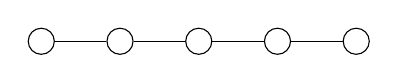
\begin{tikzpicture}
\foreach \i[count=\j from -1] in {0,...,4} {
    \node[circle,draw] (\i) at (\i,0) {};
    \ifnum\i=0\relax\else
        \draw (\j) -- (\i);
    \fi
}
\end{tikzpicture}

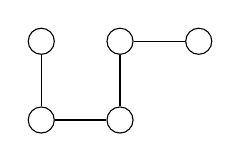
\begin{tikzpicture}
\node[circle,draw] (0) at (0,0) {};
\node[circle,draw] (1) at (0,-1) {};
\node[circle,draw] (2) at (1,-1) {};
\node[circle,draw] (3) at (1,0) {};
\node[circle,draw] (4) at (2,0) {};
\foreach \i[count=\j from 0] in {1,...,4} {
    \ifnum\i=0\relax\else
        \draw (\j) -- (\i);
    \fi
}
\end{tikzpicture}
\end{multicols}
\end{center}
\end{example}

\begin{definition}
ให้ $n$ เป็นจำนวนเต็มบวกที่มีค่าอย่างน้อย 3 \enskip \emph{กราฟวง} (cycle) $C_n$ คือกราฟที่มี $n$ vertices และมี $n$ edges ต่อกันเป็นวงรอบ
\end{definition}
%
\begin{example}
\label{ex:cycle-graph}
สองกราฟต่อไปนี้เป็น $C_5$ \enskip จะเห็นว่า แม้ว่าทั้งสองกราฟนี้จะวาดไม่เหมือนกัน แต่เราสามารถเขียนแจกแจงกราฟในรูปของคู่อันดับ $G=(V,E)$ ได้เหมือนกัน ดังนั้น สองกราฟนี้จึงเป็นกราฟเดียวกัน
\begin{center}
\begin{multicols}{2}
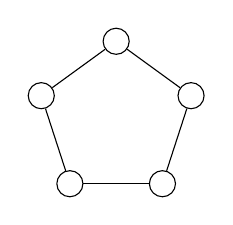
\begin{tikzpicture}
\foreach \i[count=\j from -1] in {0,...,4} {
    \node[circle,draw] (\i) at (90-72*\i:1) {};
    \ifnum\i=0\relax\else
        \draw (\j) -- (\i);
    \fi
}
\draw (4) -- (0);
\end{tikzpicture}

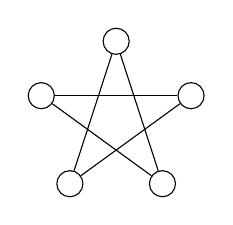
\begin{tikzpicture}
\foreach \i[count=\j from -1] in {0,...,4} {
    \node[circle,draw] (\i) at (90-144*\i:1) {};
    \ifnum\i=0\relax\else
        \draw (\j) -- (\i);
    \fi
}
\draw (4) -- (0);
\end{tikzpicture}
\end{multicols}
\end{center}
\end{example}

\subsection{Subgraphs}

\begin{definition}
ให้ $G=(V,E)$ เป็นกราฟ \enskip เรียก $G'=(V',E')$ ว่า\emph{กราฟย่อย} (subgraph) ของ $G$ หาก $V'\subseteq V$, $E'\subseteq E$, และ $\forall\set{u,v}\in E': u\in V'\wedge v\in V'$
\end{definition}
%
กล่าวอีกนัยหนึ่ง จากกราฟใดๆ เราสามารถสร้างกราฟย่อยได้ โดยการลบจุดหรือเส้นออก \enskip ทั้งนี้ หากลบจุดใดจุดหนึ่งออกจากกราฟตั้งต้น จำเป็นจะต้องลบเส้นที่ incident with จุดนั้นๆ ด้วย มิฉะนั้นเส้นดังกล่าวจะมีจุดปลายไม่ครบทั้งสองด้าน

\begin{example}
$K_5$ มี $C_5$, $K_4$, และ $L_3$ เป็น subgraphs ดังรูปที่~\ref{fig:subgraphs}

\begin{figure}
\centering
\begin{multicols}{2}
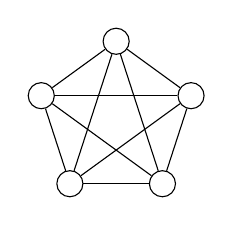
\begin{tikzpicture}
\foreach \i in {0,...,4} {
    \node[circle,draw] (\i) at (90-72*\i:1) {};
    \foreach \j in {0,...,\i} {
        \ifnum\i=\j\relax\else
        \draw (\i) -- (\j);
        \fi
    }
}
\end{tikzpicture}
\\
$K_5$ (กราฟตั้งต้น)

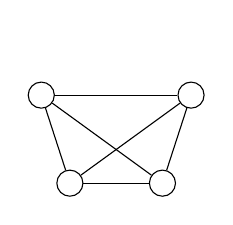
\begin{tikzpicture}
\foreach \i in {0,...,4} {
    \ifnum\i=0
        \node[circle] (\i) at (90-72*\i:1) {};
    \else
        \node[circle,draw] (\i) at (90-72*\i:1) {};
        \foreach \j in {1,...,\i} {
            \ifnum\i=\j\relax\else
            \draw (\i) -- (\j);
            \fi
        }
    \fi
}
\end{tikzpicture}
\\
$K_4$ ได้จากการลบจุดออกจาก $K_5$\\
(ซึ่งทำให้ต้องลบเส้นทิ้งไปด้วย)
\columnbreak

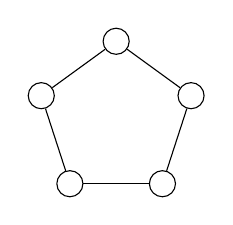
\begin{tikzpicture}
\foreach \i[count=\j from -1] in {0,...,4} {
    \node[circle,draw] (\i) at (90-72*\i:1) {};
    \ifnum\i=0\relax\else
        \draw (\j) -- (\i);
    \fi
}
\draw (4) -- (0);
\end{tikzpicture}
\\
$C_5$ ได้จากการลบเส้นออกจาก $K_5$

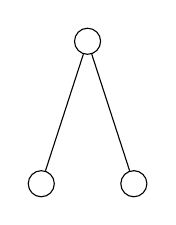
\begin{tikzpicture}
\foreach \i in {0,2,3} {
    \node[circle,draw] (\i) at (90-72*\i:1) {};
}
\draw (3) -- (0) -- (2);
\end{tikzpicture}
\\
$L_3$ ได้จากการลบทั้งจุดและเส้นออกจาก $K_5$
\end{multicols}
\caption{Subgraphs}
\label{fig:subgraphs}
\end{figure}
\end{example}

\subsection{Graph isomorphism}

จากตัวอย่างที่ผ่านๆ มา จะเห็นว่า กราฟแต่ละกราฟ อาจจะมีวิธีวาดได้หลายแบบ \enskip ในบางครั้ง อาจจะไม่ชัดเจนว่ากราฟสองกราฟที่เห็นนั้นเป็นกราฟเดียวกันหรือไม่ แต่ในเชิงทฤษฎีกราฟนั้น เราสามารถนิยามว่าเมื่อใดกราฟสองกราฟนั้น แท้จริงแล้วเป็นกราฟเดียวกัน

\begin{definition}
กราฟ $G$ และ $H$ มี\emph{สัณฐานเหมือนกัน} (isomorphic) หากสามารถตั้งชื่อ vertices ในแต่ละกราฟ แล้วทำให้เขียนกราฟทั้งสองในรูป $(V,E)$ ให้ตรงกันได้
\end{definition}
%
\begin{example}
กราฟใน Example~\ref{ex:cycle-graph} นั้น isomorphic กัน เนื่องจากเราสามารถตั้งชื่อแต่ละจุดในแต่ละกราฟดังรูปด้านล่าง แล้วทำให้เขียนแจกแจงกราฟในรูปของคู่อันดับ $G=(V,E)$ ได้เหมือนกัน กล่าวคือ
\begin{align*}
    V &= \set{1,2,3,4,5} \\
    E &= \set{\set{1,2},\set{2,3},\set{3,4},\set{4,5},\set{5,1}}
\end{align*}
\begin{center}
\begin{multicols}{2}
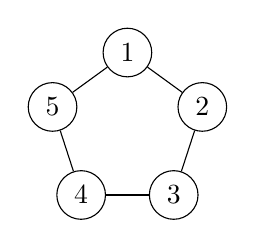
\begin{tikzpicture}
\foreach \i[count=\j from -1] in {0,...,4} {
    \node[circle,draw] (\i) at (90-72*\i:1) {\number\numexpr\i+1\relax};
    \ifnum\i=0\relax\else
        \draw (\j) -- (\i);
    \fi
}
\draw (4) -- (0);
\end{tikzpicture}

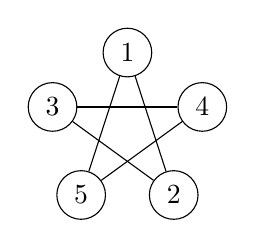
\begin{tikzpicture}
\foreach \i[count=\j from -1] in {0,...,4} {
    \node[circle,draw] (\i) at (90-144*\i:1) {\number\numexpr\i+1\relax};
    \ifnum\i=0\relax\else
        \draw (\j) -- (\i);
    \fi
}
\draw (4) -- (0);
\end{tikzpicture}
\end{multicols}
\end{center}
\end{example}

\begin{exercise}
สองกราฟต่อไปนี้ isomorphic กัน \enskip จากกราฟที่กำหนดให้ ให้กำหนดชื่อจุดแต่ละจุดในแต่ละกราฟ ที่ทำให้เขียนแจกแจงกราฟในรูปของคู่อันดับแล้ว ได้ผลลัพธ์ที่ตรงกัน
\begin{center}
\begin{multicols}{2}
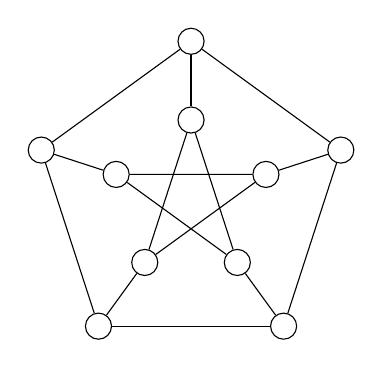
\begin{tikzpicture}
\foreach \i[count=\j from -1] in {0,...,4} {
    \node[circle,draw] (v1\i) at (90-72*\i:1) {};
    \node[circle,draw] (v2\i) at (90-72*\i:2) {};
    \draw (v1\i) -- (v2\i);
    \ifnum\i=0\relax\else
        \draw (v2\j) -- (v2\i);
    \fi
}
\draw (v24) -- (v20);
\draw (v10) -- (v12) -- (v14) -- (v11) -- (v13) -- (v10);
\end{tikzpicture}

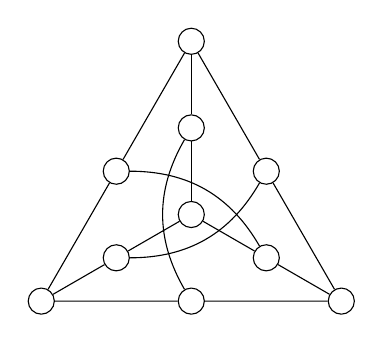
\begin{tikzpicture}
\node[circle,draw] (v0) at (0,0) {};
\foreach \j in {1,...,3} {
    \node[circle,draw] (v\j) at (150-120*\j:1.1) {};
}
\foreach \i[count=\p from 0] in {1,2} {
    \foreach \j in {0,...,2} {
        \node[circle,draw] (v\i\j) at (90-120*\j:1.1*\i) {};
        \ifnum\i=1
            \draw (v\p) -- (v\i\j);
        \else
            \draw (v\p\j) -- (v\i\j);
        \fi
    }
}
\draw (v20) -- (v1) -- (v21) -- (v2) -- (v22) -- (v3) -- (v20);
\path
    (v1) edge[bend left] (v12)
    (v2) edge[bend left] (v10)
    (v3) edge[bend left] (v11);
\end{tikzpicture}
\end{multicols}
\end{center}
\end{exercise}
